\section{Detection Mechanism}
\label{sec:detection}

In this section, we describe the main building blocks constituting the proposed detection mechanism that target detecting malicious peers and restoring benign peers satisfaction.
We start by highlighting the general overview on how the detection mechanism flows, as shown in Figure~\ref{detection-blocks}.

Then, we highlight the main differences between detecting a dropping attack behavior and detecting a manipulation/outdated chunks attack behavior, and thus, how the detection mechanism behaves.
We refer to those behaviors as \textit{Drop} attack, \textit{Manp} attack for simplicity. 
Note that the detection mechanism behaves similarly in a manipulation and outdated attack scenarios.
Afterwards, each procedure involved in the detection mechanism is detailed. 
The list of variables used throughout this section is provided in Table \ref{tab:acronyms}.

\begin{table}[ht]
\center
\caption{Acronyms}
\begin{tabular}{|c|l||c|l|}
\hline

\bf{Var.} & \bf{Description}  & \bf{Var.} & \bf{Description} \\\hline\hline
$x$ & no. of malicious peers & $\eta$ & mal. headnodes fraction\\\hline
$MN$ & malicious neighbors & $\sigma$ & satisfaction threshold\\\hline
$H_n$ & list of headnodes & $P_n$ & potential candidates list \\\hline
$\alpha$ & manipulation threshold& $F$ & familiarity of suspect \\\hline
$G$ & suspect guilt value & $\kappa$ & dropping det. allowed\\\hline
$sat$ & peer satisfaction level& $BM$ & buffer map\\\hline
\end{tabular}
\label{tab:acronyms}
\end{table}

\subsection{Mechanism Overview}
Here we describe the overall view of the detection mechanism's flow presented in Figure~\ref{detection-blocks}.
Once a detection condition is triggered by peer $b$, it sends a detection request to all peers in its neighbor list.
Afterwards, whenever a peer receives a detection request, it prepares a reply according to the request type, i.e., a \textit{Drop} or a \textit{Manp} request, 

Then, after $b$ collects all the replies, it decides according to a certain scheme, as detailed in Section~\ref{Firing_a_Complain}, whether to fire a complaint to the source or not.
If a decision is taken, $b$ sends a complaint on behalf of the participating peers in the detection request. 
The source verifies the complaint and accordingly, replies back to $b$ with the corresponding steps to follow. 
Finally, $b$ forwards the source's reply to the other participants in the complaint.

\subsection{Drop vs. Manp Detection}

On one hand, when $s$ conducts a drop attack on $b$, $b$ is not capable of detecting any malicious behavior.
Specifically, in a drop attack, $s$ never sends the actual $BM$ that represents the chunks it currently possesses, i.e., $s$ is only requesting chunks it already has.
Thus, detecting a violation in this case is not feasible.

On the other hand, in a manipulation or outdated chunks scenario, $s$ is eventually suspected as $b$ already expects the requested chunk from $s$.
Note that a peer might be overloaded due to a tight upload bandwidth or serving a lot of peers and thus, not able to serve all the requests.
Accordingly, the detection mechanism should differentiate between a malicious manipulating peer and an overloaded peer, which is discussed in Section~\ref{Detection-Trigger}.
To that end, through the rest of the section, we describe how the detection mechanism handles both cases: \textit{Drop} and \textit{Manp} detection.

\begin{figure}
 \centering
 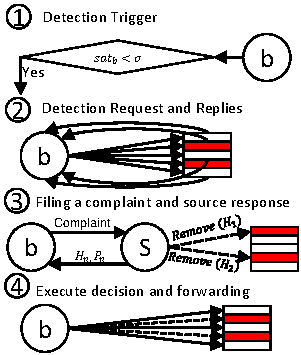
\includegraphics[width=5.5cm,height=6cm]{./Figures/detection.pdf}
  \caption{Detection mechanism process. The same process is applied for \textit{Drop} and \textit{Manp} trigger scenarios. $S$ represents the source peer. The grey entry represents a \textit{Manp} scenario. In this case, this peer does not receive a detection request.}
\label{detection-blocks} 
\end{figure}

\subsection{Detection Trigger}
\label{Detection-Trigger}
 Now we discuss how a peer decides on sending a detection request for both attack behaviors.
% In both behaviors, once $b$ decides on sending a detection request, it only sends to peers in its own neighbor list to check if those neighbors agree with it or not, disregarding the source if $b$ is a headnode.
% 
% Afterwards, as detailed in Section~\ref{Firing_a_Complain}, once $b$ receives its neighbors replies to the detection request, $b$ decides whether or not to fire a complaint to the source.

\subsubsection*{Drop trigger}
As there is no evidence of manipulation from any neighbor to $b$, the only factor that $b$ is concerned about in this attack behavior is the satisfaction threshold $\sigma$.
The satisfaction of a peer is defined as the fraction of missed chunks, i.e., the continuity of the stream according to the $Hit/Hit+miss$ chunk ratio.
In details, $b$ decides to trigger a detection request only if:
\begin{enumerate}
 \item $b$'s current satisfaction level is less than the predefined threshold such that $sat_b < \sigma$.
 \item Number of drop detections sent by $b$ in the last $1000s$ is $< \kappa$.
 \item $b$ is not currently participating in another \textit{drop} detection process.
\end{enumerate}
The latter condition guarantees that any peer can not trigger or participate in multiple detection requests in parallel as: (a) frequently sending complaints will eventually overload the source,
and (b) the source is most likely processing another peer's dropping request that is most likely to enhance $b$'s satisfaction level as we discuss in Section~\ref{complaint_source}.
Note that in a \textit{drop} attack, the detection request sent to $b$'s neighbors does not contain a certain suspect, hence, peers receiving a an empty suspect field request are aware that indeed it is a \textit{drop} request.

\subsubsection*{Manp trigger}
For each time $b$ detects a manipulation event from $s$, $b$ stores the incident in its \textit{suspicious list}.
$b$ decides to send a detection request if it was manipulated $\alpha$ times by $s$, i.e., the event counts for $s$ in $b$'s list equals $\alpha$.
Clearly, $b$ attaches the suspect ID in the detection request to its neighbors.

This condition essentially guarantees that any peer is not suspected instantly if it did not deliver the requested chunk, i.e., a benign peer might not deliver a chunk to the requester if it is already loaded due to serving other peers.
Thus, when a benign peer is incapable of serving a request of another peer, it is already aware that the event was recorded and eventually, the serving peer might be under suspicious if it did not serve the upcoming requests from the same peer.
In turn, the serving peer can assign higher priorities to serve requests for certain peers that have already manipulation logs about it.

In order to decrease the likelihood of malicious peers abusing the manipulation detection mechanism, participating peers in a \textit{Manp} request are requested to provide evidence of having the suspected peer in their neighbor list.
To obtain such evidence, whenever peer $p_1$ is adding $p_2$ to its neighboring list, $p_2$ is requested to sign its entry in $p_1$'s neighbor list.
Moreover, peers periodically request a fresh signatures from all other peers in their neighbor list.
Accordingly, only peers with such fresh signatures from $s$ are allowed to participate in the complaint, i.e, as in fact, outdated signatures might indicates connections already removed from $s$'s neighboring list.
This evidence is later needed for the source to decide about $s$, as detailed in Section~\ref{Firing_a_Complain}.

\subsection{Processing Detection Request}
Here we describe how a peer $d \in D$, where $D$ is the set of peers who received a detection request from $b$, prepares a detection reply.
As malicious peers collude with each other, they reply differently according to whether $s$ is malicious or benign.
Hence, we distinguish those two cases below. We refer to a malicious participant as $d_m$ and a benign one as $d_b$.

\subsubsection*{Benign recipient}
Once $d_b$ receives a \textit{drop} request, it replies only with its current satisfaction level $sat$.
Nevertheless, in case of a \textit{Manp} request, $d_b$ generates a reply using the following three factors:
\begin{enumerate}
 \item \textit{familiarity $F$}: where $F=1$ is $d_b$ is familiar with the suspect, $F=0$ otherwise, i.e., a boolean that states if the suspect is a current or a former neighbor of $s_b$ or not.
 \item \textit{Guilt $G$}: the number of manipulation evidences $d_b$ has against the suspect.
 Note that this number is always $<\alpha$, otherwise, $d_b$ triggers a detection request on its own.
 \item \textit{Satisfaction}: similar to \textit{drop} request, $d_b$ attaches its current satisfaction level $sat$.
\end{enumerate}


\subsubsection*{Malicious recipient}

Intuitively, $d_m$ always aim at providing the highest values that decrease the probability of $b$ reaching a decision to fire a complaint to the source, as detailed in Section~\ref{Firing_a_Complain}.
Hence, in a \textit{Drop} request, $d_m$ constantly replies with $sat=1$.
In a \textit{Manp} request, $d_m$ replies with $F=1, G=0, sat=1$ in case the $s$ is a colluding malicious peer.
Note that $d_m$ is incapable of providing fake $F$ values in its replies in case $s$ is benign due to the obligation of sending the signed proof that $s$ is indeed a neighbor of $d_m$. 
Next, we describe how $b$ processes the values provided in the detection replies in order to reach a decision about firing a complaint to the source.

\subsection{Firing a Complaint}
\label{Firing_a_Complain}
Here we discuss the procedure applied by $b$ once it receives all detection replies for a certain request, or a waiting time-out $t_{replies}$ occurs.
We assume that the source's address is publicly known and $b$ can send a complaint to the source directly whether the source is already a neighbor to $b$ or not.
\subsubsection*{Drop request}
As discussed earlier, the only factor that $b$ can consider is $sat$.
Thus, $b$ uses the following formula in order to decide about generating a complaint to the source:

\begin{align}
\label{eq:drop_satis_equation}
\sum_{i=0}^{z} sat_i/z < \sigma
\end{align}
where $z$ is the total number of the received replies. 
In other words, $b$ sends a complaint only if the average satisfaction level of its neighbors is below than the predefined satisfaction threshold $\sigma$.

To prevent malicious peers from abusing the drop detection mechanism and cause an illusion at the source that a general dissatisfaction is detected, the following conditions are applied:
\begin{enumerate}
 \item Each peer can at most generate or participate in maximum $\kappa$ drop complaints to the source per $1000s$.
 \item No simultaneous generation or participation in more than one complaint is allowed to any peer, i.e., once $d$ is engaged in a detection process, it should wait till the final decision is reached.
\end{enumerate}
Although those conditions guarantee that malicious peers can not abuse the drop detection mechanism,
however, benign peers also have the same constraints which might reside in a benign peer not able to eventually complain to the source.
For those reasons, as we further elaborate on Section~\ref{complaint_source}, once a drop detection complaint reaches the source, the fraction of headnodes replaced is large in order to maximize the likelihood of affecting a large fraction of the overlay, specially for peers who might not be able to complain to the source at the moment.

\subsubsection*{Manp request}
In this simpler case where a certain suspect exists, $b$ decides to fire a complaint if the following conditions hold:

\begin{align}
\label{eq:drop_familiarity_equation}
\sum_{i=0}^{z} F_i > z/2
\end{align}
The condition in \ref{eq:drop_familiarity_equation} assures that at least more than half of the participant peers have information about the suspect, i.e., the suspect is an entry in their neighbor list.
Next, for \textit{familiar} peers with the suspect, the aggregated \textit{Guilt} reported value must be greater than the maximum calculated value that can be reported by familiar peers, as stated in ~\ref{eq:drop_guilt_equation}.

\begin{align}
\label{eq:drop_guilt_equation}
\sum_{i=0}^{z} G_i > \sum_{i=0}^{z} F_i*(\alpha-1)/2
\end{align}
Nevertheless, the same condition for \textit{Drop} detection in \ref{eq:drop_guilt_equation} is also considered in a \textit{Manp} type.
The reason for considering the satisfaction factor is to assure that the participating peers are currently unsatisfied, i.e., $d_b$ might have manipulation event for $s$ in their \textit{suspicious list} , however, $d_b$ is satisfied through other peers and no gain for it from firing a complaint and overload the source.

\subsubsection*{Firing a complaint to the source}

Once $b$ decides on firing a complaint according to the aforementioned conditions, $b$ generates a complaint message to the source.
In a \textit{Manp} scenario, $b$ attaches the following information to the complaint message: (a) IDs of \textit{familiar} peers, (b) evidences of manipulation gathered from the replies, (c) per reply values of $G,sat$ and (d) suspect's $s$ ID.
While in a \textit{Drop} scenario $b$ attaches: (a) IDs of all participating peers, and (b) $sat$ value in each reply.

\subsection{Processing a Complaint at the Source}
\label{complaint_source}
At this point the source receives a complaint from $b$, the source decides on the next procedure depending on whether the complaint is a \textit{Drop} or a \textit{Manp}.
Note that the source can identify the request's type based on the suspect field, i.e., in case of no suspect attached, it is indeed a \textit{Drop} complaint.

\subsubsection*{Manp request}
We start with the simpler case of receiving a \textit{Manp} request. 
The source executes the following steps:
\begin{enumerate}
 \item Requests the neighboring list of $s$ to validate the familiarity of peers participating in the complaint, as discussed in Section~\ref{Detection-Trigger}.
 \item If the above check is passed, the source removes the suspect $s$ from its neighbor list.
 \item Saves the free entry in its list (after removing $s$) for $b$ to connect and be a headnode.
 Accordingly, all the peers participating in the complaint will have a direct headnode ($b$) which remarkably enhances their satisfaction level.
 \item $s$ is added to a blacklist, i.e., $s$ is not allowed to be a headnode again.
 \item Generates a \textit{Complaint Reply} to $b$ confirming blacklisting $s$.
\end{enumerate}

\subsubsection*{Drop request}
Now we consider the \textit{Drop} complaint. The source conducts the following procedure:
\begin{enumerate}
 \item Divides the set of participating peers into two sets $H_n$ and $P_n$, where $H_n$ is assigned as the set of peers participating in the complaint that are already headnodes.
 \item Removes all peers in $H_n$ from its neighbor set.
 \item Randomly connects to another $|H_n|$ peers. 
 The reason for not connecting to a fraction of the participating peers in the complaint is to avoid the probability that malicious peers are abusing the detection mechanism in order to get promoted to headnodes.
 \item Adds peers (excluding peers in $H_n$) from its neighbor list to $P_n$, where $P_n = NeighborList\setminus H_n$ ($NeighborList$ is the set of peers in a neighbor list).
 \item Sends a \textit{Complaint Reply} to $b$ containing $H_n$ and $P_n$.
\end{enumerate}

\subsection{Processing a Complaint Reply \& Forwarding}

Finally, when $b$ receives the \textit{complaint Reply} from the source, $b$ performs the following procedure,
which again differs based on the complaint type (\textit{Drop} or \textit{Manp}).
In a \textit{Manp} scenario, $b$ executes the following procedure:
\begin{enumerate}
 \item Disconnects and blacklist the suspect.
 \item Connects to the source, if, due to any other reason, the connection is not possible, $b$ connects to another random peer (excluding peers in $b$'s blacklist).
 \item Forwards the \textit{Complaint Reply} to all peers who agree about $s$ being malicious, i.e., familiar peers with $G > 0$.
\end{enumerate}
Finally, the participating peers performs step 1 and 2 once they receive the forwarded reply.

For a \textit{Drop} scenario, $b$ follows the next procedure:
\begin{enumerate}
 \item Disconnects from all peers in $H_n$. Note that peers in $H_n$ are not expelled from $b$'s neighbor list due to the fact that those peers are not proven malicious.
 \item Connects to $|H_n|$ peers from $P_n$, in case $|H_n|>|P_n|$, peers connect to $|P_n|+(|H_n|-|P_n|)random peers$.
\end{enumerate}
Similarly, $b$ forwards the complaint to the other participants, who in turn execute steps 1 and 2.

\subsection{General Notes}
The detection mechanism does not aim at expelling peers from the system.
The reason behind that is the \textit{Drop} adversarial behavior, where basically benign peers are equally probable to be removed from the source's neighbor list as malicious ones.
Thus, by keeping those peers in the system, the impact on such peers is minimized, i.e., they are neither entirely expelled from the system nor even blacklisted at the peers participating in the complaint neighbor list.
In general, the main target of the detection mechanism in a \textit{Drop} case is to enhance the peers satisfaction level while minimizing: (a) peers replacements (through minimizing the number of detection requests initiated), (b) detection overhead, and (c) malicious peers chances to abuse the detection mechanism.

Unlike in a \textit{Drop} detection complaint, in a \textit{Manp} complaint, peers proved malicious through out the detection process are eventually located at distant positions from the source (due to the removals occue once those peers are detected)..
Hence, the reliance on those peers to deliver chunks to other peers is significantly minimized compared to headnodes peers or even headnodes neighbors (which positively impacts the overlay's satisfaction in case those peers are indeed malicious or due to low bandwidth, CPU resources or even an unreliable network connection).
In the following section, we evaluate our mechanism's performance and accuracy, along with highlighting the attack's severity.



